\documentclass[12pt]{article}
\usepackage[a4paper, top=0.4in, bottom=0.3in, left=0.3in, right=0.3in]{geometry}
\usepackage{graphicx}
\usepackage{subcaption}
\usepackage{listings}
\usepackage{xcolor}
\usepackage{float}
\usepackage{lmodern}
\usepackage[T1]{fontenc}
\usepackage{setspace}
\usepackage{array}
\usepackage{booktabs}
\usepackage{tabularx}
\usepackage{titlesec}
\usepackage{hyperref}

% Sans-serif throughout (like the AI PDF)
\renewcommand{\familydefault}{\sfdefault}

% Hyperref colors
\hypersetup{colorlinks=false}

% Colors matching AI PDF style
\definecolor{rcblue}{RGB}{30, 100, 200}
\definecolor{rcpurple}{RGB}{100, 60, 160}
\definecolor{codegreen}{rgb}{0,0.6,0}
\definecolor{codegray}{rgb}{0.5,0.5,0.5}
\definecolor{codepurple}{rgb}{0.58,0,0.82}
\definecolor{backcolour}{rgb}{0.97,0.97,0.97}

% Code listing style
\lstdefinestyle{mystyle}{
    backgroundcolor=\color{backcolour},
    commentstyle=\color{codegreen},
    keywordstyle=\color{blue}\bfseries,
    numberstyle=\small\color{codegray},
    stringstyle=\color{codepurple},
    basicstyle=\ttfamily\footnotesize,
    breaklines=true,
    captionpos=b,
    keepspaces=true,
    numbers=left,
    numbersep=8pt,
    showspaces=false,
    showstringspaces=false,
    tabsize=4,
    xleftmargin=16pt,
    xrightmargin=4pt,
    frame=single,
    framesep=4pt,
    rulecolor=\color{gray!40}
}
\lstset{style=mystyle}

% Section title formatting
\titleformat{\section}[block]
  {\large\bfseries}
  {\thesection.}
  {0.5em}
  {}
\titlespacing*{\section}{0pt}{18pt}{6pt}

\setlength{\parindent}{0pt}
\setlength{\parskip}{10pt}

\begin{document}

% ============================================================
% TITLE PAGE
% ============================================================
\begin{titlepage}
\centering
% \vspace*{-10pt}

{\fontsize{33pt}{36pt}\selectfont\bfseries Digital Image Processing Practical}\\[20pt]

\includegraphics[width=0.75\textwidth]{college_logo.png}\\[26pt]

{\fontsize{28pt}{26pt}\selectfont\bfseries\color{rcblue} Ramanujan College}\\[10pt]

{\fontsize{25pt}{20pt}\selectfont\bfseries\color{rcblue} DSC-19: Digital Image Processing}\\[10pt]

{\fontsize{25pt}{22pt}\selectfont\bfseries\color{rcblue} Semester-7}\\[10pt]

{\fontsize{20pt}{22pt}\selectfont\bfseries\color{rcblue} (2026-27)}\\[80pt]


\begin{tabular}{p{0.60\textwidth} p{0.48\textwidth}}
{\large\bfseries Submitted By:} & {\large\bfseries Submitted To:} \\[6pt]
{\large\bfseries $\sim$Ratnesh Kumar} & {\large\bfseries $\sim$ Dr. Arun Aggarwal} \\[3pt]
{\large\bfseries 20231432 (23020570034)} & {\large\bfseries Assistant Professor} \\[3pt]
{\large\bfseries B.Sc.\ (Hons.) CS / VII} & {\large\bfseries Department of Computer Science} \\
\end{tabular}

\end{titlepage}

% ============================================================
% ACKNOWLEDGEMENT PAGE
% ============================================================
\newpage
\begin{center}
{\fontsize{26pt}{32pt}\selectfont\bfseries Acknowledgement}
\end{center}

\vspace{16pt}
\setstretch{1.5}
{\large
I would like to take this opportunity to acknowledge everyone who has helped me in every stage of this practical work.

I am deeply indebted to my Digital Image Processing Professor, \textbf{Dr. Arun Aggarwal}, Assistant Professor, Department of Computer Science, Ramanujan College, for the valuable guidance, constant encouragement, and suggestions in completing this practical. The completion of this practical was possible under their guidance and support.

I am also thankful to the \textbf{Principal, Ramanujan College}, and the \textbf{Department of Computer Science} for providing the necessary infrastructure and academic environment. I extend my appreciation to all faculty members and laboratory staff who assisted me during the course of this work.

I am also very thankful to my parents and my friends who have boosted me up morally with their continuous support.

At last but not least, I am very thankful to God almighty for showering his blessings upon me.
}
\setstretch{1}

% ============================================================
% INDEX PAGE
% ============================================================
\newpage
\begin{center}
{\fontsize{35pt}{30pt}\selectfont\bfseries\itshape\color{rcblue} Index}
\end{center}

\vspace{6pt}

\renewcommand{\arraystretch}{0.9}
\begin{tabularx}{\textwidth}{|>{\centering\bfseries\large}p{1.5cm}|>{\large}X|}
\hline
\large\bfseries S.no & \centering\large\bfseries Topic \tabularnewline
\hline
1. & \textbf{Basic Image Operations} \\
   & a. Read and display image \\
   & b. Resize a given image \\
   & c. Convert a given color image into a corresponding gray-scale image \\
   & d. Convert a given color/gray-scale image into black \& white image and draw the image profile \\
   & e. Separate a given color image into three R, G \& B planes \\
   & f. Create a color image using separate three R, G and B planes \\
   & g. Write given 2-D data in image file \\
\hline
2. & \textbf{Point Processing Methods} \\
   & a. Obtain negative image \\
   & b. Obtain flip image \\
   & c. Thresholding \\
   & d. Contrast stretching \\
\hline
3. & \textbf{Image Arithmetic Operations} \\
   & a. Addition of two images \\
   & b. Subtract one image from other image \\
   & c. Calculate mean value of image \\
   & d. Different brightness by changing mean value \\
\hline
4. & \textbf{Image Logical Operations} \\
   & a. AND operation between two images \\
   & b. OR operation between two images \\ 
   & c. Calculate intersection of two images \\
   & d. Water marking using X-OR operation \\
   & e. NOT operation (negative image) \\
\hline
5. & \textbf{Histogram Calculation and Equalization} \\
   & a. Using inbuilt function \\
   & b. Without using inbuilt function \\
\hline
6. & \textbf{Geometric Transformations} \\
   & a. Translation \\
   & b. Scaling \\
   & c. Rotation \\
   & d. Shrinking \\
   & e. Zooming \\
\hline
7. & \textbf{Noise Models and Restoration} \\
   & a. Image restoration \\
   & b. Remove salt and pepper noise \\
   & c. Minimize Gaussian noise \\
   & d. Median filter and Wiener filter \\
\hline
8. & \textbf{Spatial Filtering} \\
   & a. Understand 1-D and 2-D convolution process \\
   & b. Use 3$x$3 mask for low pass filter and high pass filter \\
\hline
9. & \textbf{Frequency Domain Filtering} \\
   & a. Apply FFT on given image \\
   & b. Perform low pass and high pass filtering in frequency domain \\
   & c. Apply IFFT to reconstruct image \\
\hline
10. & \textbf{Edge Detection} \\
   & Edge detection using different edge detection mask \\
\hline
11. & \textbf{Morphological Operations} \\
   & Image morphological operations: erosion and dilation \\
\hline
\end{tabularx}

% ============================================================
% PRACTICALS BODY
% ============================================================
\newpage
\pagenumbering{arabic}
\setstretch{1.15}
%--- Practical 1 ---
\section*{\large\bfseries Practical 1: Basic Image Operations}
\addcontentsline{toc}{section}{Practical 1: Basic Image Operations}

\textbf{\large Code:}

% \textbf{\normalsize practical1.py}
\begin{lstlisting}[language=Python]
import cv2
import numpy as np
import matplotlib.pyplot as plt
import os

# Create result directory
os.makedirs("result/program1", exist_ok=True)

# Generate a sample image
img = np.zeros((300, 300, 3), dtype=np.uint8)
img[50:250, 50:250] = [0, 0, 255]  # Blue square
img[100:200, 100:200] = [0, 255, 0]  # Green square
cv2.imwrite("result/program1/input.jpg", img)

# a. Read and display image
img = cv2.imread("result/program1/input.jpg")

# b. Resize a given image
resized = cv2.resize(img, (150, 150))
cv2.imwrite("result/program1/resized.jpg", resized)

# c. Convert a given color image into a corresponding gray-scale image
gray = cv2.cvtColor(img, cv2.COLOR_BGR2GRAY)
cv2.imwrite("result/program1/grayscale.jpg", gray)

# d. Convert a given color/gray-scale image into black & white image
_, bw = cv2.threshold(gray, 127, 255, cv2.THRESH_BINARY)
cv2.imwrite("result/program1/black_white.jpg", bw)

# Image profile
row_profile = gray.mean(axis=1)
col_profile = gray.mean(axis=0)

# e. Separate a given color image into three R, G & B planes
b, g, r = cv2.split(img)
cv2.imwrite("result/program1/b_plane.jpg", b)
cv2.imwrite("result/program1/g_plane.jpg", g)
cv2.imwrite("result/program1/r_plane.jpg", r)

# f. Create a color image using separate three R, G and B planes
merged = cv2.merge((b, g, r))
cv2.imwrite("result/program1/merged_rgb.jpg", merged)

# g. Write given 2-D data in image file
cv2.imwrite("result/program1/output_2d.jpg", gray)

plt.plot(row_profile, label='Row profile')
plt.plot(col_profile, label='Column profile')
plt.title('d. Image profile')
plt.xlabel('Index')
plt.ylabel('Mean intensity')
plt.legend()
plt.grid(True)
plt.savefig("result/program1/image_profile.png")
plt.close()

print("All outputs saved to result/program1/")
\end{lstlisting}

\vspace{8pt}
\textbf{\large Output:}

\begin{figure}[H]
\centering
\begin{subfigure}[b]{0.31\textwidth}
  \centering
  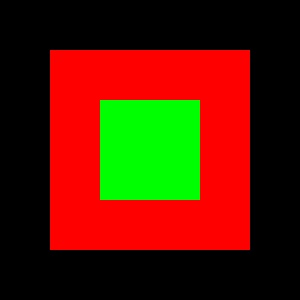
\includegraphics[width=\textwidth,height=3.3cm,keepaspectratio]{result/program1/input.jpg}
  \caption{Input Image}
\end{subfigure}\hfill
\begin{subfigure}[b]{0.31\textwidth}
  \centering
  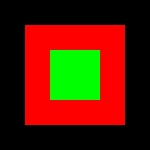
\includegraphics[width=\textwidth,height=3.3cm,keepaspectratio]{result/program1/resized.jpg}
  \caption{Resized Image (150x150)}
\end{subfigure}\hfill
\begin{subfigure}[b]{0.31\textwidth}
  \centering
  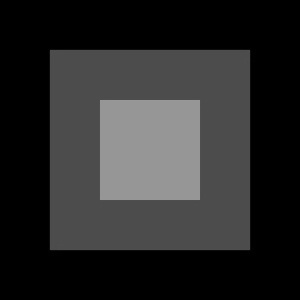
\includegraphics[width=\textwidth,height=3.3cm,keepaspectratio]{result/program1/grayscale.jpg}
  \caption{Grayscale Image}
\end{subfigure}
\vspace{6pt}

\begin{subfigure}[b]{0.31\textwidth}
  \centering
  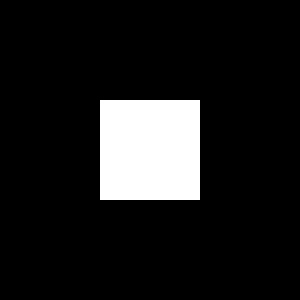
\includegraphics[width=\textwidth,height=3.3cm,keepaspectratio]{result/program1/black_white.jpg}
  \caption{Black \& White}
\end{subfigure}\hfill
\begin{subfigure}[b]{0.31\textwidth}
  \centering
  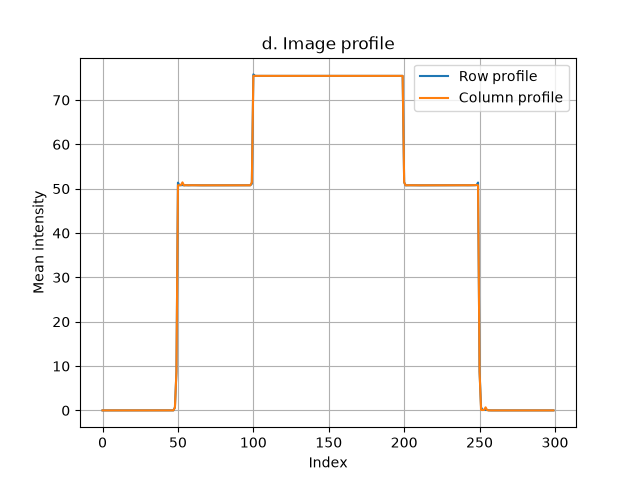
\includegraphics[width=\textwidth,height=3.3cm,keepaspectratio]{result/program1/image_profile.png}
  \caption{Image Profile Plot}
\end{subfigure}\hfill
\begin{subfigure}[b]{0.31\textwidth}
  \centering
  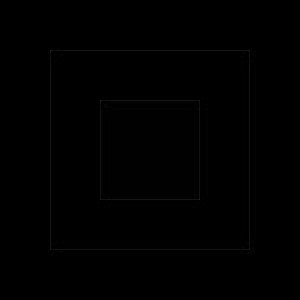
\includegraphics[width=\textwidth,height=3.3cm,keepaspectratio]{result/program1/b_plane.jpg}
  \caption{B (Blue) Plane}
\end{subfigure}
\vspace{6pt}

\begin{subfigure}[b]{0.31\textwidth}
  \centering
  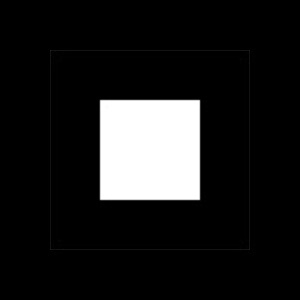
\includegraphics[width=\textwidth,height=3.3cm,keepaspectratio]{result/program1/g_plane.jpg}
  \caption{G (Green) Plane}
\end{subfigure}\hfill
\begin{subfigure}[b]{0.31\textwidth}
  \centering
  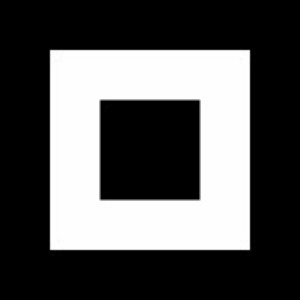
\includegraphics[width=\textwidth,height=3.3cm,keepaspectratio]{result/program1/r_plane.jpg}
  \caption{R (Red) Plane}
\end{subfigure}\hfill
\begin{subfigure}[b]{0.31\textwidth}
  \centering
  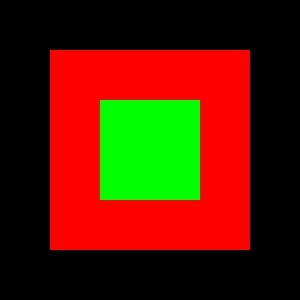
\includegraphics[width=\textwidth,height=3.3cm,keepaspectratio]{result/program1/merged_rgb.jpg}
  \caption{Merged RGB Image}
\end{subfigure}
\vspace{6pt}

\begin{subfigure}[b]{0.31\textwidth}
  \centering
  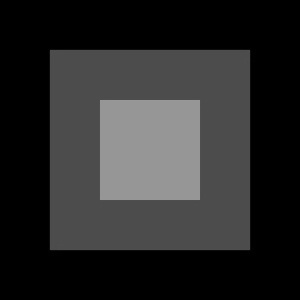
\includegraphics[width=\textwidth,height=3.3cm,keepaspectratio]{result/program1/output_2d.jpg}
  \caption{2D Data Output}
\end{subfigure}
\end{figure}

\newpage
%--- Practical 2 ---
\section*{\large\bfseries Practical 2: Point Processing Methods}
\addcontentsline{toc}{section}{Practical 2: Point Processing Methods}

\textbf{\large Code:}

% \textbf{\normalsize practical2.py}
\begin{lstlisting}[language=Python]
import cv2
import numpy as np
import os

os.makedirs("result/program2", exist_ok=True)

# Generate synthetic image
img = np.linspace(0, 255, 256, dtype=np.uint8).reshape(16, 16)
img = cv2.resize(img, (256, 256), interpolation=cv2.INTER_NEAREST)
cv2.imwrite("result/program2/original.jpg", img)

# a. Negative image
negative = 255 - img
cv2.imwrite("result/program2/negative.jpg", negative)

# b. Flip image
hor_flipped = cv2.flip(img, 1)  # horizontal flip
cv2.imwrite("result/program2/horizontal_flipped.jpg", hor_flipped)
ver_flipped = cv2.flip(img, 0)  # vertical flip
cv2.imwrite("result/program2/vertical_flipped.jpg", ver_flipped)

# c. Thresholding
_, thresholded = cv2.threshold(img, 127, 255, cv2.THRESH_BINARY)
cv2.imwrite("result/program2/thresholded.jpg", thresholded)

# d. Contrast stretching
min_val, max_val = np.min(img), np.max(img)
stretched = ((img - min_val) / (max_val - min_val) * 255).astype(np.uint8)
cv2.imwrite("result/program2/contrast_stretched.jpg", stretched)

print("All outputs saved to result/program2/")
\end{lstlisting}

\vspace{8pt}
\textbf{\large Output:}

\begin{figure}[H]
\centering
\begin{subfigure}[b]{0.31\textwidth}
  \centering
  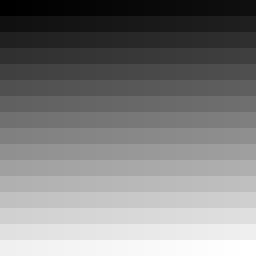
\includegraphics[width=\textwidth,height=3.3cm,keepaspectratio]{result/program2/original.jpg}
  \caption{Original Image}
\end{subfigure}\hfill
\begin{subfigure}[b]{0.31\textwidth}
  \centering
  
\includegraphics[width=\textwidth,height=3.3cm,keepaspectratio]{result/program2/negative.jpg}
  \caption{Negative Image}
\end{subfigure}\hfill
\begin{subfigure}[b]{0.31\textwidth}
  \centering
  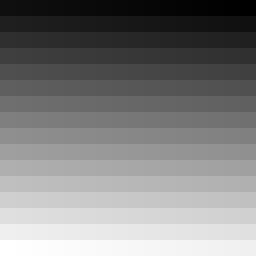
\includegraphics[width=\textwidth,height=3.3cm,keepaspectratio]{result/program2/horizontal_flipped.jpg}
  \caption{Horizontal Flipped}
\end{subfigure}
\vspace{6pt}

\begin{subfigure}[b]{0.31\textwidth}
  \centering
  
\includegraphics[width=\textwidth,height=3.3cm,keepaspectratio]{result/program2/vertical_flipped.jpg}
  \caption{Vertical Flipped}
\end{subfigure}\hfill
\begin{subfigure}[b]{0.31\textwidth}
  \centering
  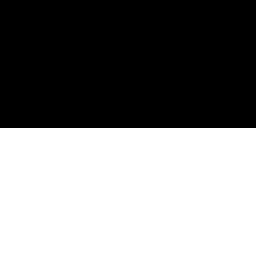
\includegraphics[width=\textwidth,height=3.3cm,keepaspectratio]{result/program2/thresholded.jpg}
  \caption{Thresholded Image}
\end{subfigure}\hfill
\begin{subfigure}[b]{0.31\textwidth}
  \centering
  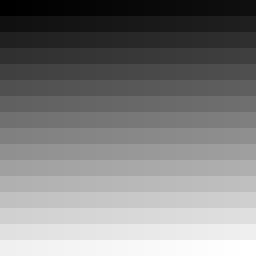
\includegraphics[width=\textwidth,height=3.3cm,keepaspectratio]{result/program2/contrast_stretched.jpg}
  \caption{Contrast Stretched}
\end{subfigure}
\end{figure}


\newpage
%--- Practical 3 ---
\section*{\large\bfseries Practical 3: Image Arithmetic Operations}
\addcontentsline{toc}{section}{Practical 3: Image Arithmetic Operations}

\textbf{\large Code:}

% \textbf{\normalsize practical3.py}
\begin{lstlisting}[language=Python]
import cv2
import numpy as np
import os

os.makedirs("result/program3", exist_ok=True)

# Create sample images
img1 = np.zeros((256, 256), dtype=np.uint8)
cv2.rectangle(img1, (50, 50), (150, 150), 100, -1)

img2 = np.zeros((256, 256), dtype=np.uint8)
cv2.circle(img2, (150, 150), 70, 150, -1)

cv2.imwrite("result/program3/image1.jpg", img1)
cv2.imwrite("result/program3/image2.jpg", img2)

# a. Addition of two images
added = cv2.add(img1, img2)
cv2.imwrite("result/program3/added.jpg", added)

# b. Subtract one image from other image
subtracted1 = cv2.subtract(img1, img2)
subtracted2 = cv2.subtract(img2, img1)
cv2.imwrite("result/program3/subtracted_img1_img2.jpg", subtracted1)
cv2.imwrite("result/program3/subtracted_img2_img1.jpg", subtracted2)

# c. Calculate mean value of image
mean1 = np.mean(img1)
mean2 = np.mean(img2)
with open("result/program3/mean_values.txt", "w") as f:
    f.write(f"Mean of image1: {mean1}\n")
    f.write(f"Mean of image2: {mean2}\n")

# d. Different brightness by changing mean value
# Use calculated mean values (mean1, mean2) to adjust brightness
# Brighten img1 by adding mean2, darken by subtracting mean2
brightened = cv2.add(img1, int(mean2))
darkened = cv2.subtract(img1, int(mean2))

cv2.imwrite("result/program3/brightened.jpg", brightened)
cv2.imwrite("result/program3/darkened.jpg", darkened)

print("All outputs saved to result/program3/")
\end{lstlisting}

\vspace{8pt}
\textbf{\large Output:}

\textbf{\normalsize Calculated Mean Intensities:}
\begin{lstlisting}[style=mystyle, numbers=none]
Mean of image1: 15.56549072265625
Mean of image2: 35.186004638671875
\end{lstlisting}
\vspace{6pt}

\begin{figure}[H]
\centering
\begin{subfigure}[b]{0.31\textwidth}
  \centering
  
\includegraphics[width=\textwidth,height=3.3cm,keepaspectratio]{result/program3/image1.jpg}
  \caption{Image 1}
\end{subfigure}\hfill
\begin{subfigure}[b]{0.31\textwidth}
  \centering
  
\includegraphics[width=\textwidth,height=3.3cm,keepaspectratio]{result/program3/image2.jpg}
  \caption{Image 2}
\end{subfigure}\hfill
\begin{subfigure}[b]{0.31\textwidth}
  \centering
  
\includegraphics[width=\textwidth,height=3.3cm,keepaspectratio]{result/program3/added.jpg}
  \caption{Addition of Images}
\end{subfigure}
\vspace{6pt}

\begin{subfigure}[b]{0.31\textwidth}
  \centering
  
\includegraphics[width=\textwidth,height=3.3cm,keepaspectratio]{result/program3/subtracted_img1_img2.jpg}
  \caption{Subtracted (Img1 - Img2)}
\end{subfigure}\hfill
\begin{subfigure}[b]{0.31\textwidth}
  \centering
  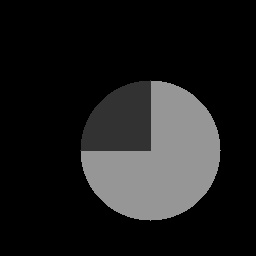
\includegraphics[width=\textwidth,height=3.3cm,keepaspectratio]{result/program3/subtracted_img2_img1.jpg}
  \caption{Subtracted (Img2 - Img1)}
\end{subfigure}\hfill
\begin{subfigure}[b]{0.31\textwidth}
  \centering
  
\includegraphics[width=\textwidth,height=3.3cm,keepaspectratio]{result/program3/brightened.jpg}
  \caption{Brightened Image (+Mean)}
\end{subfigure}
\vspace{6pt}

\begin{subfigure}[b]{0.31\textwidth}
  \centering
  
\includegraphics[width=\textwidth,height=3.3cm,keepaspectratio]{result/program3/darkened.jpg}
  \caption{Darkened Image (-Mean)}
\end{subfigure}\hfill
\end{figure}

\newpage
%--- Practical 4 ---
\section*{\large\bfseries Practical 4: Image Logical Operations}
\addcontentsline{toc}{section}{Practical 4: Image Logical Operations}

\textbf{\large Code:}

% \textbf{\normalsize practical4.py}
\begin{lstlisting}[language=Python]
import cv2
import numpy as np
import os

os.makedirs("result/program4", exist_ok=True)

# Create sample binary images
img1 = np.zeros((200, 200), dtype=np.uint8)
cv2.rectangle(img1, (50, 50), (120, 120), 255, -1)

img2 = np.zeros((200, 200), dtype=np.uint8)
cv2.circle(img2, (100, 100), 50, 255, -1)

cv2.imwrite("result/program4/image1.jpg", img1)
cv2.imwrite("result/program4/image2.jpg", img2)

# a. AND operation between two images
and_img = cv2.bitwise_and(img1, img2)
cv2.imwrite("result/program4/and.jpg", and_img)

# b. OR operation between two images
or_img = cv2.bitwise_or(img1, img2)
cv2.imwrite("result/program4/or.jpg", or_img)

# c. Calculate intersection of two images
intersection = cv2.bitwise_and(img1, img2)
cv2.imwrite("result/program4/intersection.jpg", intersection)

# d. Water marking using X-OR operation
logo = np.zeros((200, 200), dtype=np.uint8)
cv2.putText(logo, "DIP", (40, 110), cv2.FONT_HERSHEY_SIMPLEX, 1.5, 255, 3)
watermarked = cv2.bitwise_xor(img1, logo)
extracted = cv2.bitwise_xor(watermarked, logo)
cv2.imwrite("result/program4/logo.jpg", logo)
cv2.imwrite("result/program4/watermarked_xor.jpg", watermarked)
cv2.imwrite("result/program4/extracted_xor.jpg", extracted)

# e. NOT operation (negative image)
not_img1 = cv2.bitwise_not(img1)
cv2.imwrite("result/program4/not_image1.jpg", not_img1)

print("All outputs saved to result/program4/")
\end{lstlisting}

\vspace{8pt}
\textbf{\large Output:}

\begin{figure}[H]
\centering
\begin{subfigure}[b]{0.31\textwidth}
  \centering
  
\includegraphics[width=\textwidth,height=3.3cm,keepaspectratio]{result/program4/image1.jpg}
  \caption{Image 1}
\end{subfigure}\hfill
\begin{subfigure}[b]{0.31\textwidth}
  \centering
  
\includegraphics[width=\textwidth,height=3.3cm,keepaspectratio]{result/program4/image2.jpg}
  \caption{Image 2}
\end{subfigure}\hfill
\begin{subfigure}[b]{0.31\textwidth}
  \centering
  
\includegraphics[width=\textwidth,height=3.3cm,keepaspectratio]{result/program4/and.jpg}
  \caption{AND Operation}
\end{subfigure}
\vspace{6pt}

\begin{subfigure}[b]{0.31\textwidth}
  \centering
  
\includegraphics[width=\textwidth,height=3.3cm,keepaspectratio]{result/program4/or.jpg}
  \caption{OR Operation}
\end{subfigure}\hfill
\begin{subfigure}[b]{0.31\textwidth}
  \centering
  
\includegraphics[width=\textwidth,height=3.3cm,keepaspectratio]{result/program4/intersection.jpg}
  \caption{Intersection}
\end{subfigure}\hfill
\begin{subfigure}[b]{0.31\textwidth}
  \centering
  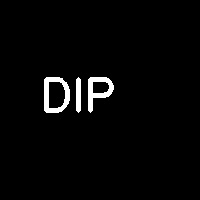
\includegraphics[width=\textwidth,height=3.3cm,keepaspectratio]{result/program4/logo.jpg}
  \caption{Logo Image}
\end{subfigure}
\vspace{6pt}

\begin{subfigure}[b]{0.31\textwidth}
  \centering
  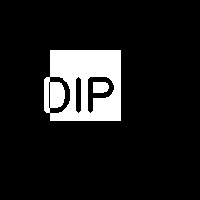
\includegraphics[width=\textwidth,height=3.3cm,keepaspectratio]{result/program4/watermarked_xor.jpg}
  \caption{Watermarked Image (XOR)}
\end{subfigure}\hfill
\begin{subfigure}[b]{0.31\textwidth}
  \centering
  
\includegraphics[width=\textwidth,height=3.3cm,keepaspectratio]{result/program4/extracted_xor.jpg}
  \caption{Extracted Watermark (XOR)}
\end{subfigure}\hfill
\begin{subfigure}[b]{0.31\textwidth}
  \centering
  
\includegraphics[width=\textwidth,height=3.3cm,keepaspectratio]{result/program4/not_image1.jpg}
  \caption{NOT Operation (Negative)}
\end{subfigure}
\end{figure}


\newpage
%--- Practical 5 ---
\section*{\large\bfseries Practical 5: Histogram Calculation and Equalization}
\addcontentsline{toc}{section}{Practical 5: Histogram Calculation and Equalization}

\textbf{\large Code:}

% \textbf{\normalsize practical5.py}
\begin{lstlisting}[language=Python]
import cv2
import numpy as np
import os

os.makedirs("result/program5", exist_ok=True)

# Load image
img = cv2.imread("input.jpg")
if img is None:
    for p in ["result/program5/input_ref.jpg", "result/program7/input_ref.jpg", "result/program1/input.jpg"]:
        img = cv2.imread(p)
        if img is not None:
            break
if img is None:
    img = np.zeros((256, 256, 3), dtype=np.uint8)
    cv2.rectangle(img, (50, 50), (200, 200), (120, 180, 220), -1)

gray = cv2.cvtColor(img, cv2.COLOR_BGR2GRAY)
cv2.imwrite("result/program5/input_img.jpg", gray)
cv2.imwrite("result/program5/grayscale.jpg", gray)

# a
eq_builtin = cv2.equalizeHist(gray)
cv2.imwrite("result/program5/equalized_builtin.jpg", eq_builtin)

# b
cdf = cv2.calcHist([gray], [0], None, [256], [0, 256]).flatten().cumsum()
cdf_min = cdf[cdf != 0].min() if np.any(cdf != 0) else 0
cdf_max = cdf[-1]
denom = cdf_max - cdf_min
if denom <= 0:
    lut = np.zeros(256, dtype=np.uint8)
else:
    lut = ((cdf - cdf_min) * 255.0 / denom)
    lut = np.clip(lut, 0, 255).astype(np.uint8)
img_eq_manual = lut[gray]
cv2.imwrite("result/program5/equalized_manual.jpg", img_eq_manual)

print("All outputs saved to result/program5/")
\end{lstlisting}

\vspace{8pt}
\textbf{\large Output:}

\begin{figure}[H]
\centering
\begin{subfigure}[b]{0.24\textwidth}
  \centering
  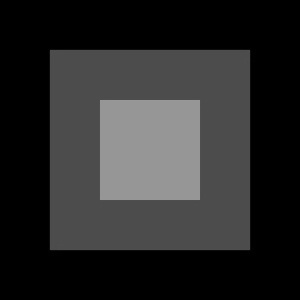
\includegraphics[width=\textwidth,height=3cm,keepaspectratio]{result/program5/input_img.jpg}
  \caption{Input Image}
\end{subfigure}\hfill
\begin{subfigure}[b]{0.24\textwidth}
  \centering
  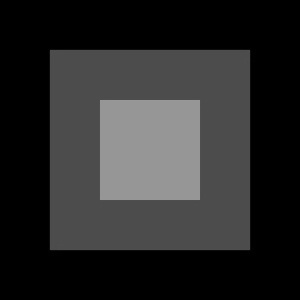
\includegraphics[width=\textwidth,height=3cm,keepaspectratio]{result/program5/grayscale.jpg}
  \caption{Grayscale Image}
\end{subfigure}\hfill
\begin{subfigure}[b]{0.24\textwidth}
  \centering
  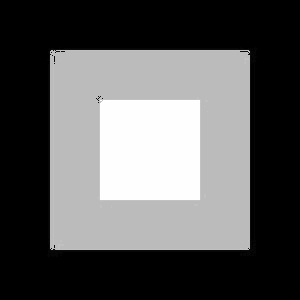
\includegraphics[width=\textwidth,height=3cm,keepaspectratio]{result/program5/equalized_builtin.jpg}
  \caption{Equalized (Built-in)}
\end{subfigure}\hfill
\begin{subfigure}[b]{0.24\textwidth}
  \centering
  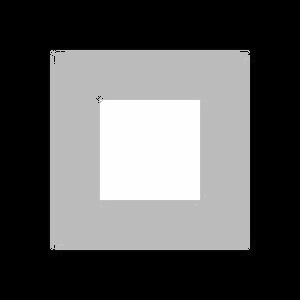
\includegraphics[width=\textwidth,height=3cm,keepaspectratio]{result/program5/equalized_manual.jpg}
  \caption{Equalized (Manual)}
\end{subfigure}
\end{figure}


\newpage
%--- Practical 6 ---
\section*{\large\bfseries Practical 6: Geometric Transformations}
\addcontentsline{toc}{section}{Practical 6: Geometric Transformations}

\textbf{\large Code:}

% \textbf{\normalsize practical6.py}
\begin{lstlisting}[language=Python]
import cv2
import numpy as np
import os

os.makedirs("result/program6", exist_ok=True)

# Create sample image
img = np.zeros((150, 150, 3), dtype=np.uint8)
cv2.rectangle(img, (30, 30), (90, 90), (0, 255, 0), -1)
cv2.imwrite("result/program6/original.jpg", img)

# a. Translation
h, w = img.shape[:2]
M = np.float32([[1, 0, 50], [0, 1, 30]])
translated = cv2.warpAffine(img, M, (w, h))
cv2.imwrite("result/program6/translated.jpg", translated)

# b. Scaling
scaled = cv2.resize(img, None, fx=1.5, fy=1.5, interpolation=cv2.INTER_LINEAR)
cv2.imwrite("result/program6/scaled.jpg", scaled)

# c. Rotation
M_rot = cv2.getRotationMatrix2D((w/2, h/2), 45, 1)
rotated = cv2.warpAffine(img, M_rot, (w, h))
cv2.imwrite("result/program6/rotated.jpg", rotated)

# d. Shrinking
shrunk = cv2.resize(img, None, fx=0.5, fy=0.5, interpolation=cv2.INTER_AREA)
cv2.imwrite("result/program6/shrunk.jpg", shrunk)

# e. Zooming
zoomed = cv2.resize(img, None, fx=2.0, fy=2.0, interpolation=cv2.INTER_CUBIC)
cv2.imwrite("result/program6/zoomed.jpg", zoomed)

print("All outputs saved to result/program6/")
\end{lstlisting}

\vspace{8pt}
\textbf{\large Output:}

\begin{figure}[H]
\centering
\begin{subfigure}[b]{0.31\textwidth}
  \centering
  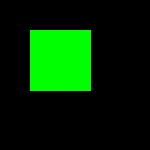
\includegraphics[width=\textwidth,height=2.4cm,keepaspectratio]{result/program6/original.jpg}
  \caption{Original Image}
\end{subfigure}\hfill
\begin{subfigure}[b]{0.31\textwidth}
  \centering
  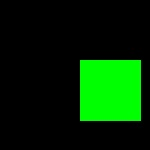
\includegraphics[width=\textwidth,height=2.4cm,keepaspectratio]{result/program6/translated.jpg}
  \caption{Translated Image}
\end{subfigure}\hfill
\begin{subfigure}[b]{0.31\textwidth}
  \centering
  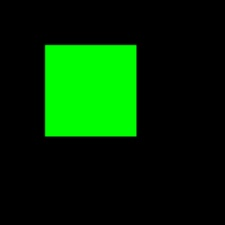
\includegraphics[width=\textwidth,height=2.4cm,keepaspectratio]{result/program6/scaled.jpg}
  \caption{Scaled Image}
\end{subfigure}
\vspace{2pt}

\begin{subfigure}[b]{0.31\textwidth}
  \centering
  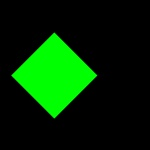
\includegraphics[width=\textwidth,height=2.4cm,keepaspectratio]{result/program6/rotated.jpg}
  \caption{Rotated ($45^\circ$)}
\end{subfigure}\hfill
\begin{subfigure}[b]{0.31\textwidth}
  \centering
  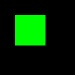
\includegraphics[width=\textwidth,height=2.4cm,keepaspectratio]{result/program6/shrunk.jpg}
  \caption{Shrunk Image}
\end{subfigure}\hfill
\begin{subfigure}[b]{0.31\textwidth}
  \centering
  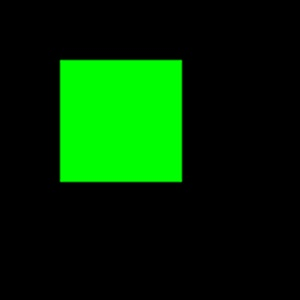
\includegraphics[width=\textwidth,height=2.4cm,keepaspectratio]{result/program6/zoomed.jpg}
  \caption{Zoomed Image}
\end{subfigure}
\end{figure}

\newpage
%--- Practical 7 ---
\section*{\large\bfseries Practical 7: Noise Models and Restoration}
\addcontentsline{toc}{section}{Practical 7: Noise Models and Restoration}

\textbf{\large Code:}

% \textbf{\normalsize practical7.py}
\begin{lstlisting}[language=Python]
import cv2
import numpy as np
import os
import random
from scipy.signal import wiener

random.seed(42)
np.random.seed(42)

os.makedirs("result/program7", exist_ok=True)

# Find input image
img = None
for p in ["input.jpg", "result/program1/input.jpg", "result/program5/grayscale.jpg", "result/program5/input_img.jpg"]:
    if os.path.exists(p):
        img = cv2.imread(p, 0)
        if img is not None:
            break
if img is None:
    img = np.zeros((256, 256), dtype=np.uint8)
    cv2.rectangle(img, (50, 50), (200, 200), 150, -1)

cv2.imwrite("result/program7/original.jpg", img)

# Salt & Pepper
noisy_sp = img.copy().astype(np.float32)
total = img.size
s_vs_p = 0.5; amount = 0.05
n_s = int(np.ceil(amount*total*s_vs_p)); n_p = int(np.ceil(amount*total*(1-s_vs_p)))
for _ in range(n_s):
    r,c = random.randint(0,img.shape[0]-1), random.randint(0,img.shape[1]-1)
    noisy_sp[r,c]=255
for _ in range(n_p):
    r,c = random.randint(0,img.shape[0]-1), random.randint(0,img.shape[1]-1)
    noisy_sp[r,c]=0
noisy_sp = np.clip(noisy_sp,0,255).astype(np.uint8)
cv2.imwrite("result/program7/salt_pepper_noisy.jpg", noisy_sp)
med = cv2.medianBlur(noisy_sp,3)
cv2.imwrite("result/program7/median_filtered.jpg", med)

# Gaussian
g = np.random.normal(0,10,img.shape)
ng = np.clip(img.astype(float)+g,0,255).astype(np.uint8)
cv2.imwrite("result/program7/gaussian_noisy.jpg", ng)
gf = cv2.GaussianBlur(ng,(5,5),0)
cv2.imwrite("result/program7/gaussian_filtered.jpg", gf)

# Wiener filter (for Gaussian noise restoration)
# scipy.signal.wiener applies adaptive Wiener filtering
wiener_filtered = wiener(ng.astype(np.float32), mysize=5, noise=None)
wiener_filtered = np.clip(wiener_filtered, 0, 255).astype(np.uint8)
cv2.imwrite("result/program7/wiener_filtered.jpg", wiener_filtered)

# Also apply Wiener filter to salt & pepper noise for comparison
wiener_sp = wiener(noisy_sp.astype(np.float32), mysize=5, noise=None)
wiener_sp = np.clip(wiener_sp, 0, 255).astype(np.uint8)
cv2.imwrite("result/program7/wiener_sp_filtered.jpg", wiener_sp)

print("All outputs saved to result/program7/")
\end{lstlisting}

\vspace{8pt}
\textbf{\large Output:}

\begin{figure}[H]
\centering
\begin{subfigure}[b]{0.31\textwidth}
  \centering
  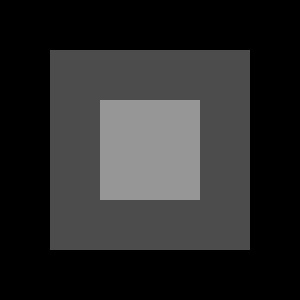
\includegraphics[width=\textwidth,height=3.3cm,keepaspectratio]{result/program7/original.jpg}
  \caption{Original Image}
\end{subfigure}\hfill
\begin{subfigure}[b]{0.31\textwidth}
  \centering
  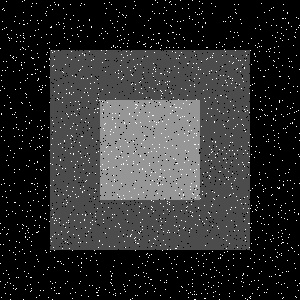
\includegraphics[width=\textwidth,height=3.3cm,keepaspectratio]{result/program7/salt_pepper_noisy.jpg}
  \caption{Salt \& Pepper Noise}
\end{subfigure}\hfill
\begin{subfigure}[b]{0.31\textwidth}
  \centering
  
\includegraphics[width=\textwidth,height=3.3cm,keepaspectratio]{result/program7/median_filtered.jpg}
  \caption{Median Filtered}
\end{subfigure}

\vspace{6pt}

\begin{subfigure}[b]{0.31\textwidth}
  \centering
  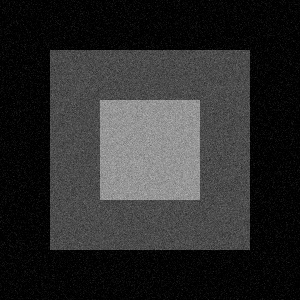
\includegraphics[width=\textwidth,height=3.3cm,keepaspectratio]{result/program7/gaussian_noisy.jpg}
  \caption{Gaussian Noise}
\end{subfigure}\hfill
\begin{subfigure}[b]{0.31\textwidth}
  \centering
  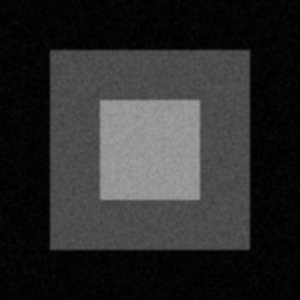
\includegraphics[width=\textwidth,height=3.3cm,keepaspectratio]{result/program7/gaussian_filtered.jpg}
  \caption{Gaussian Filtered}
\end{subfigure}\hfill
\begin{subfigure}[b]{0.31\textwidth}
  \centering
  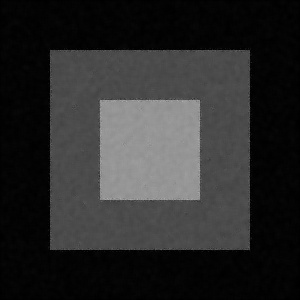
\includegraphics[width=\textwidth,height=3.3cm,keepaspectratio]{result/program7/wiener_filtered.jpg}
  \caption{Wiener Filtered (Gaussian)}
\end{subfigure}
\vspace{6pt}
\begin{subfigure}[b]{0.31\textwidth}
  \centering
 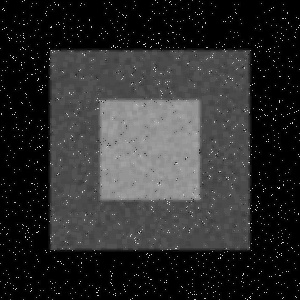
\includegraphics[width=\textwidth,height=3.3cm,keepaspectratio]{result/program7/wiener_sp_filtered.jpg}
  \caption{Wiener Filtered (Salt \& Pepper)}
\end{subfigure}\hfill

\end{figure}


\newpage
%--- Practical 8 ---
\section*{\large\bfseries Practical 8: Spatial Filtering}
\addcontentsline{toc}{section}{Practical 8: Spatial Filtering}

\textbf{\large Code:}

% \textbf{\normalsize practical8.py}
\begin{lstlisting}[language=Python]
import cv2
import numpy as np
import os
import random

random.seed(42)
np.random.seed(42)

os.makedirs("result/program8", exist_ok=True)

# Load image
img = None
for p in ["input.jpg", "result/program1/input.jpg", "result/program5/grayscale.jpg"]:
    if os.path.exists(p):
        img = cv2.imread(p, 0)
        if img is not None: break
if img is None:
    img = np.zeros((128,128),dtype=np.uint8); cv2.rectangle(img,(20,20),(100,100),255,-1)

cv2.imwrite("result/program8/original.jpg", img)
imgf = img.astype(np.float32)

# 1D conv
k1 = np.array([1,2,1],dtype=np.float32)/4.0
conv1d = np.convolve(imgf[0,:], k1, mode='same')

# LP
klp = np.ones((3,3),dtype=np.float32)/9.0
lp = cv2.filter2D(imgf,-1,klp)
cv2.imwrite("result/program8/low_pass.jpg", lp.astype(np.uint8))
# HP
khp = np.array([[-1,-1,-1],[-1,8,-1],[-1,-1,-1]],dtype=np.float32)
hp = cv2.filter2D(imgf,-1,khp)
hp = np.clip(hp,0,255).astype(np.uint8)
cv2.imwrite("result/program8/high_pass.jpg", hp)

print("All outputs saved to result/program8/")
\end{lstlisting}

\vspace{8pt}
\textbf{\large Output:}

\begin{figure}[H]
\centering
\begin{subfigure}[b]{0.31\textwidth}
  \centering
  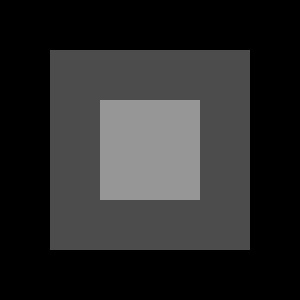
\includegraphics[width=\textwidth,height=3.3cm,keepaspectratio]{result/program8/original.jpg}
  \caption{Original Image}
\end{subfigure}\hfill
\begin{subfigure}[b]{0.31\textwidth}
  \centering
  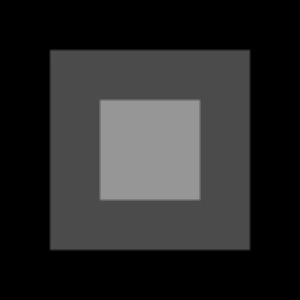
\includegraphics[width=\textwidth,height=3.3cm,keepaspectratio]{result/program8/low_pass.jpg}
  \caption{Low Pass Filtered}
\end{subfigure}\hfill
\begin{subfigure}[b]{0.31\textwidth}
  \centering
  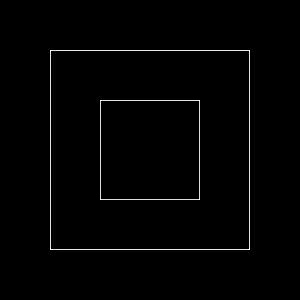
\includegraphics[width=\textwidth,height=3.3cm,keepaspectratio]{result/program8/high_pass.jpg}
  \caption{High Pass Filtered}
\end{subfigure}
\end{figure}


\newpage
%--- Practical 9 ---
\section*{\large\bfseries Practical 9: Frequency Domain Filtering}
\addcontentsline{toc}{section}{Practical 9: Frequency Domain Filtering}

\textbf{\large Code:}

% \textbf{\normalsize practical9.py}
\begin{lstlisting}[language=Python]
import cv2
import numpy as np
import os

os.makedirs("result/program9", exist_ok=True)

img = None
for p in ["input.jpg","result/program1/input.jpg","result/program5/grayscale.jpg"]:
    if os.path.exists(p):
        img = cv2.imread(p,0)
        if img is not None: break
if img is None:
    img = np.zeros((256,256),dtype=np.uint8); cv2.rectangle(img,(50,50),(200,200),255,-1)

cv2.imwrite("result/program9/original.jpg", img)

f = np.fft.fft2(img); fshift = np.fft.fftshift(f)
mag = 20*np.log(np.abs(fshift)+1e-10)
mag = np.clip(mag,0,255).astype(np.uint8)
cv2.imwrite("result/program9/magnitude_spectrum.png", mag)

r,c = img.shape; cr,cc = r//2,c//2
mask_lp = np.zeros((r,c),np.uint8); cv2.circle(mask_lp,(cc,cr),30,255,-1)
mask_hp = cv2.bitwise_not(mask_lp)

fsl = fshift*(mask_lp/255.0); fsh = fshift*(mask_hp/255.0)
il = np.abs(np.fft.ifft2(np.fft.ifftshift(fsl))); ih = np.abs(np.fft.ifft2(np.fft.ifftshift(fsh)))
il = np.clip(il,0,255).astype(np.uint8); ih = np.clip(ih,0,255).astype(np.uint8)
cv2.imwrite("result/program9/low_pass_filtered.jpg", il)
cv2.imwrite("result/program9/high_pass_filtered.jpg", ih)

print("All outputs saved to result/program9/")
\end{lstlisting}

\vspace{8pt}
\textbf{\large Output:}

\begin{figure}[H]
\centering
\begin{subfigure}[b]{0.24\textwidth}
  \centering
  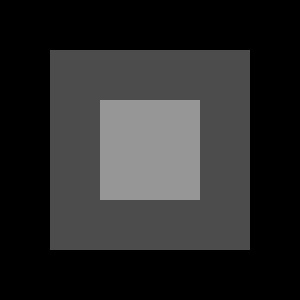
\includegraphics[width=\textwidth,height=3.3cm,keepaspectratio]{result/program9/original.jpg}
  \caption{Original Image}
\end{subfigure}\hfill
\begin{subfigure}[b]{0.24\textwidth}
  \centering
  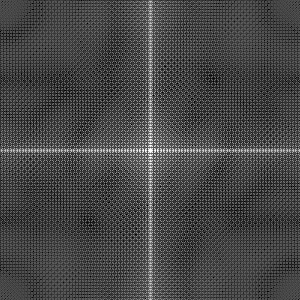
\includegraphics[width=\textwidth,height=3.3cm,keepaspectratio]{result/program9/magnitude_spectrum.png}
  \caption{Magnitude Spectrum}
\end{subfigure}\hfill
\begin{subfigure}[b]{0.24\textwidth}
  \centering
  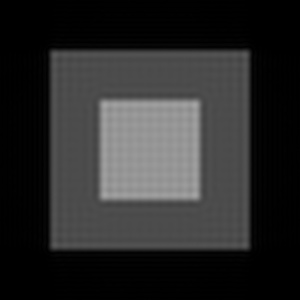
\includegraphics[width=\textwidth,height=3.3cm,keepaspectratio]{result/program9/low_pass_filtered.jpg}
  \caption{Low Pass Filtered}
\end{subfigure}
\begin{subfigure}[b]{0.24\textwidth}
  \centering
  
\includegraphics[width=\textwidth,height=3.3cm,keepaspectratio]{result/program9/high_pass_filtered.jpg}
  \caption{High Pass Filtered}
\end{subfigure}\hfill
\end{figure}


\newpage
%--- Practical 10 ---
\section*{\large\bfseries Practical 10: Edge Detection}
\addcontentsline{toc}{section}{Practical 10: Edge Detection}

\textbf{\large Code:}

% \textbf{\normalsize practical10.py}
\begin{lstlisting}[language=Python]
import cv2
import numpy as np
import os

os.makedirs("result/program10", exist_ok=True)

img = None
for p in ["input.jpg","result/program1/input.jpg","result/program5/grayscale.jpg"]:
    if os.path.exists(p):
        img = cv2.imread(p,0)
        if img is not None: break
if img is None:
    img = np.zeros((256,256),dtype=np.uint8); cv2.rectangle(img,(50,50),(200,200),255,-1)

cv2.imwrite("result/program10/original.jpg", img)

# Sobel
sx = cv2.Sobel(img,cv2.CV_64F,1,0,ksize=3); sy = cv2.Sobel(img,cv2.CV_64F,0,1,ksize=3)
sob = np.clip(np.hypot(sx,sy),0,255).astype(np.uint8)

# Prewitt
kx=np.array([[1,1,1],[0,0,0],[-1,-1,-1]]); ky=np.array([[-1,0,1],[-1,0,1],[-1,0,1]])
px=cv2.filter2D(img,-1,kx); py=cv2.filter2D(img,-1,ky)
pre = np.clip(np.hypot(px.astype(float),py.astype(float)),0,255).astype(np.uint8)

# Roberts
rx=np.array([[1,0],[0,-1]]); ry=np.array([[0,1],[-1,0]])
rxv=cv2.filter2D(img,-1,rx); ryv=cv2.filter2D(img,-1,ry)
rob = np.clip(np.hypot(rxv.astype(float),ryv.astype(float)),0,255).astype(np.uint8)

# Canny
can = cv2.Canny(img,50,150)
cv2.imwrite("result/program10/sobel.jpg", sob)
cv2.imwrite("result/program10/prewitt.jpg", pre)
cv2.imwrite("result/program10/roberts.jpg", rob)
cv2.imwrite("result/program10/canny.jpg", can)

print("All outputs saved to result/program10/")
\end{lstlisting}

\vspace{8pt}
\textbf{\large Output:}

\begin{figure}[H]
\centering
\begin{subfigure}[b]{0.31\textwidth}
  \centering
  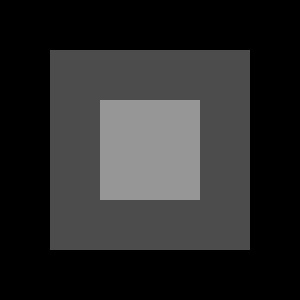
\includegraphics[width=\textwidth,height=3.3cm,keepaspectratio]{result/program10/original.jpg}
  \caption{Original Image}
\end{subfigure}\hfill
\begin{subfigure}[b]{0.31\textwidth}
  \centering
  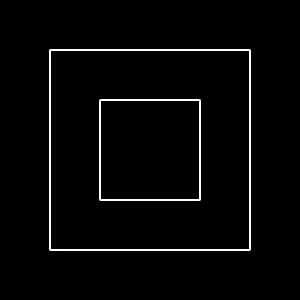
\includegraphics[width=\textwidth,height=3.3cm,keepaspectratio]{result/program10/sobel.jpg}
  \caption{Sobel Operator}
\end{subfigure}\hfill
\begin{subfigure}[b]{0.31\textwidth}
  \centering
  
\includegraphics[width=\textwidth,height=3.3cm,keepaspectratio]{result/program10/prewitt.jpg}
  \caption{Prewitt Operator}
\end{subfigure}

\vspace{6pt}

\begin{subfigure}[b]{0.31\textwidth}
  \centering
  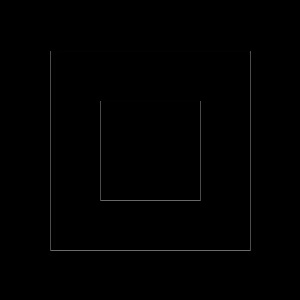
\includegraphics[width=\textwidth,height=3.3cm,keepaspectratio]{result/program10/roberts.jpg}
  \caption{Roberts Operator}
\end{subfigure}\hfill
\begin{subfigure}[b]{0.31\textwidth}
  \centering
  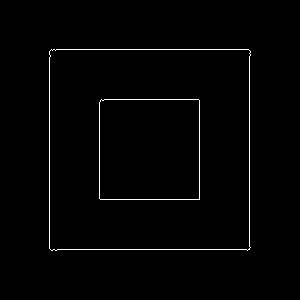
\includegraphics[width=\textwidth,height=3.3cm,keepaspectratio]{result/program10/canny.jpg}
  \caption{Canny Edge Detection}
\end{subfigure}\hfill
\end{figure}


\newpage
%--- Practical 11 ---
\section*{\large\bfseries Practical 11: Morphological Operations}
\addcontentsline{toc}{section}{Practical 11: Morphological Operations}

\textbf{\large Code:}

% \textbf{\normalsize practical11.py}
\begin{lstlisting}[language=Python]
import cv2
import numpy as np
import os

os.makedirs("result/program11", exist_ok=True)

img = None
for p in ["input.jpg","result/program1/input.jpg","result/program5/grayscale.jpg"]:
    if os.path.exists(p):
        img = cv2.imread(p,0)
        if img is not None: break
if img is None:
    img = np.zeros((200,200),dtype=np.uint8); cv2.putText(img,'DIP',(40,120),cv2.FONT_HERSHEY_SIMPLEX,2.5,255,5)

cv2.imwrite("result/program11/original.jpg", img)

k = np.ones((5,5),np.uint8)
er = cv2.erode(img,k,iterations=1)
di = cv2.dilate(img,k,iterations=1)
op = cv2.morphologyEx(img,cv2.MORPH_OPEN,k)
cl = cv2.morphologyEx(img,cv2.MORPH_CLOSE,k)
cv2.imwrite("result/program11/erosion.jpg", er)
cv2.imwrite("result/program11/dilation.jpg", di)
cv2.imwrite("result/program11/opening.jpg", op)
cv2.imwrite("result/program11/closing.jpg", cl)

print("All outputs saved to result/program11/")
\end{lstlisting}

\vspace{6pt}
\textbf{\large Output:}

\begin{figure}[H]
\centering
\begin{subfigure}[b]{0.31\textwidth}
  \centering
  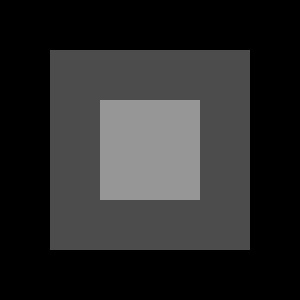
\includegraphics[width=\textwidth,height=3.3cm,keepaspectratio]{result/program11/original.jpg}
  \caption{Original Image}
\end{subfigure}\hfill
\begin{subfigure}[b]{0.31\textwidth}
  \centering
  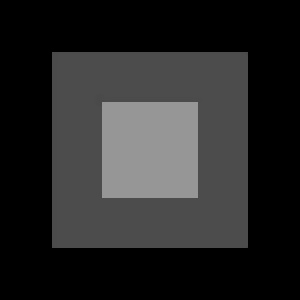
\includegraphics[width=\textwidth,height=3.3cm,keepaspectratio]{result/program11/erosion.jpg}
  \caption{Erosion}
\end{subfigure}\hfill
\begin{subfigure}[b]{0.31\textwidth}
  \centering
  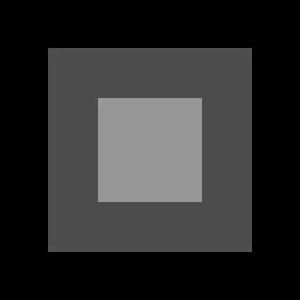
\includegraphics[width=\textwidth,height=3.3cm,keepaspectratio]{result/program11/dilation.jpg}
  \caption{Dilation}
\end{subfigure}

\vspace{6pt}

\begin{subfigure}[b]{0.31\textwidth}
  \centering
  
\includegraphics[width=\textwidth,height=3.3cm,keepaspectratio]{result/program11/opening.jpg}
  \caption{Opening}
\end{subfigure}\hfill
\begin{subfigure}[b]{0.31\textwidth}
  \centering
  
\includegraphics[width=\textwidth,height=3.3cm,keepaspectratio]{result/program11/closing.jpg}
  \caption{Morphological Closing}
\end{subfigure}\hfill
\end{figure}

\end{document}
